\documentclass[]{article}
\usepackage[utf8]{inputenc}
\usepackage{graphicx}
\usepackage{textcomp}
\usepackage{fullpage}
\usepackage{float}
\usepackage{listings}

\usepackage{verbatim}
\usepackage{hyperref}


\title{Deep Learning Assignment 4}
\author{Nikita Teplitskiy}

\begin{document}
\maketitle

The goal of this assignment was to create a pair of convolutional neural network designed to categorize images from the CIFAR-10 and CIFAR-100 data sets. 

\section{CIFAR-10 Model}

The initial model used for the CIFAR-10 categorizer was based on the ``toy ResNet'' described in the TensorFlow/Keras documentation. This model worked moderately well achieving 76.9\% top-1 accuracy and 98.3\% top-5 accuracy. It consisted of 7 convolutional layers, 3 residual layers, and 2 dense layers resulting in a total of 223,242 trainable parameters. Convergence would occur within 15 epochs. This model suffers from significant overfit that was improved by adding regularization to some layers.  

The second model attempted was from [2] which was a conventional convolutional network utilizing 4 convolutional layer, 2 dense layers, and max pooling where appropriate. The claimed benefit of this model was its relatively small size and memory footprint which would improve training speed. Unfortunately, the model presented in the paper does not appear to be the model they derived results from. The model as described and illustrated is so much smaller than the predicted model size and provides awful results. 

The third design was a convolution only design from the paper [3] ``Striving for Simplicity: The All Convolutional Net'' that dispersed with any dense layers employing a purely convolutional design. This model performed adequately well achieving a top-1 and top-5 accuracy of 61.0\% and 94.5\% respectively. Curiously, when the author suggested dropout was added to the model, the top-5 accuracy started out very high and achieved 100\% within a few epochs. Given the sub 10\% true accuracy of the model, this erroneous result was due to misconfiguration. 

\section{CIFAR-100 Model}

The first model used for the CIFAR-100 dataset was a modification of the third model mentioned previously. The only change made was alterting the output dimension to 100 categories and adding additional regularization. This model achieved mediocre results, reaching 68.9\% top-5. 

The second model was an enlarged version of the ResNet that was tested for the CIFAR-10 model. An additional convolutional block was added and the sizes of the dense layers were adjusted. This model achieved 79.8\% accuracy but further improvement was curtailed by limited training time. 

The third model used was lifted directly from a tutorial [4] as I have zero success with the previous two models. This model was fast and allowed me to diagnose some major issues the prevented the previous models from working as expected. This model achieves a subpar top-5 accuracy of 67.4\% but made up for it in speed and simplicity.   

\section{Conclusions}

Further exprimentation is needed in saving and restoring models. TensorBoard would be more convenient for monitoring results. Need to set up CUDA environment as CPU training times are getting excessive.

\section{References}

1. \url{https://www.tensorflow.org/guide/keras/functional\#a_toy_resnet_model} \\
2.  Calik, Demirci. Cifar-10 Image Classification with ConvolutionalNeural Networks For Embedded Systems \\
3. Springenberg, Dosovitskiy, Brox, Riedmiller. STRIVING FOR SIMPLICITY: THE ALL CONVOLUTIONAL NET \\
4. \url{https://www.machinecurve.com/index.php/2020/02/09/how-to-build-a-convnet-for-cifar-10-and-cifar-100-classification-with-keras/}

\begin{figure}[H]
    \centering
    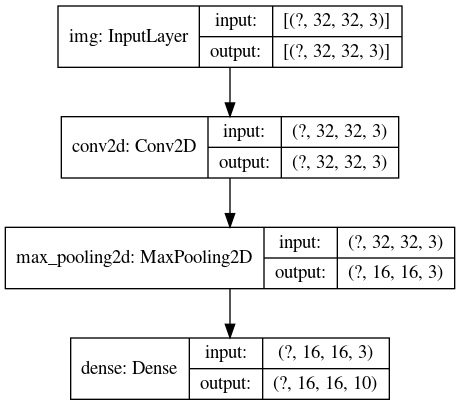
\includegraphics[width=0.47\textwidth]{cifar10_model.png}
    \caption{CIFAR-10 ResNet Structure}
\end{figure}

\begin{figure}[H]
    \centering
    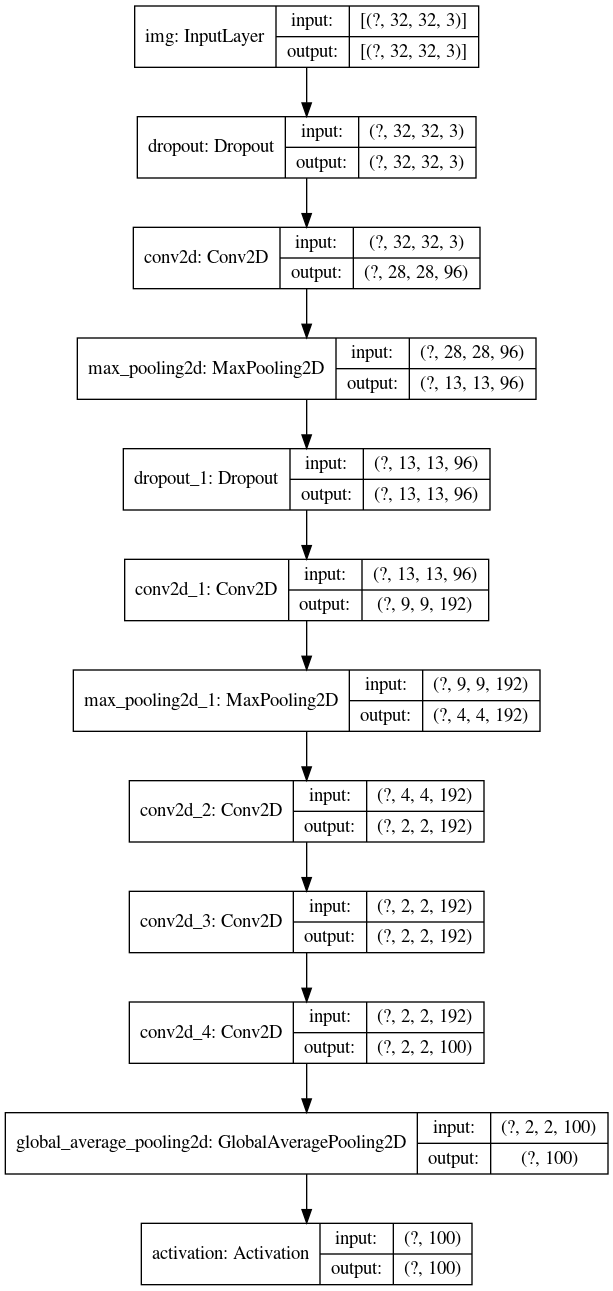
\includegraphics[width=0.5\textwidth]{cifar100_model.png}
    \caption{CIFAR-100 ResNet Structure}
\end{figure}

\newpage
\onecolumn


\newpage
\section{CIFAR-10 Model}
\lstinputlisting[breaklines=true,language=Python]{a4.py}
\newpage
\section{CIFAR-100 Model}
\lstinputlisting[breaklines=true,language=Python]{a4-cifar-100.py}
\newpage
\section{CIFAR Dataset Loader}
\lstinputlisting[breaklines=true,language=Python]{LoadCIFAR.py}

\end{document}
